\chapter{Accept Test Logs} \label{a:results}
This appendix includes a condensed version of the logs printed with every test of the full setup. The different test scenarios are distinguished in each section.

\section{Straight Line-of-Sight}
The test is made with the antennas pointing directly towards each other. The distance between the antennas is $d=\SI{5.4}{\meter}$. The start position is \SI{10}{\degree}, the end position is \SI{150}{\degree} and the increase is \SI{20}{\degree}. The following figure \ref{fig:a2_1} shows the setup:
\begin{figure}[H]
    \centering
    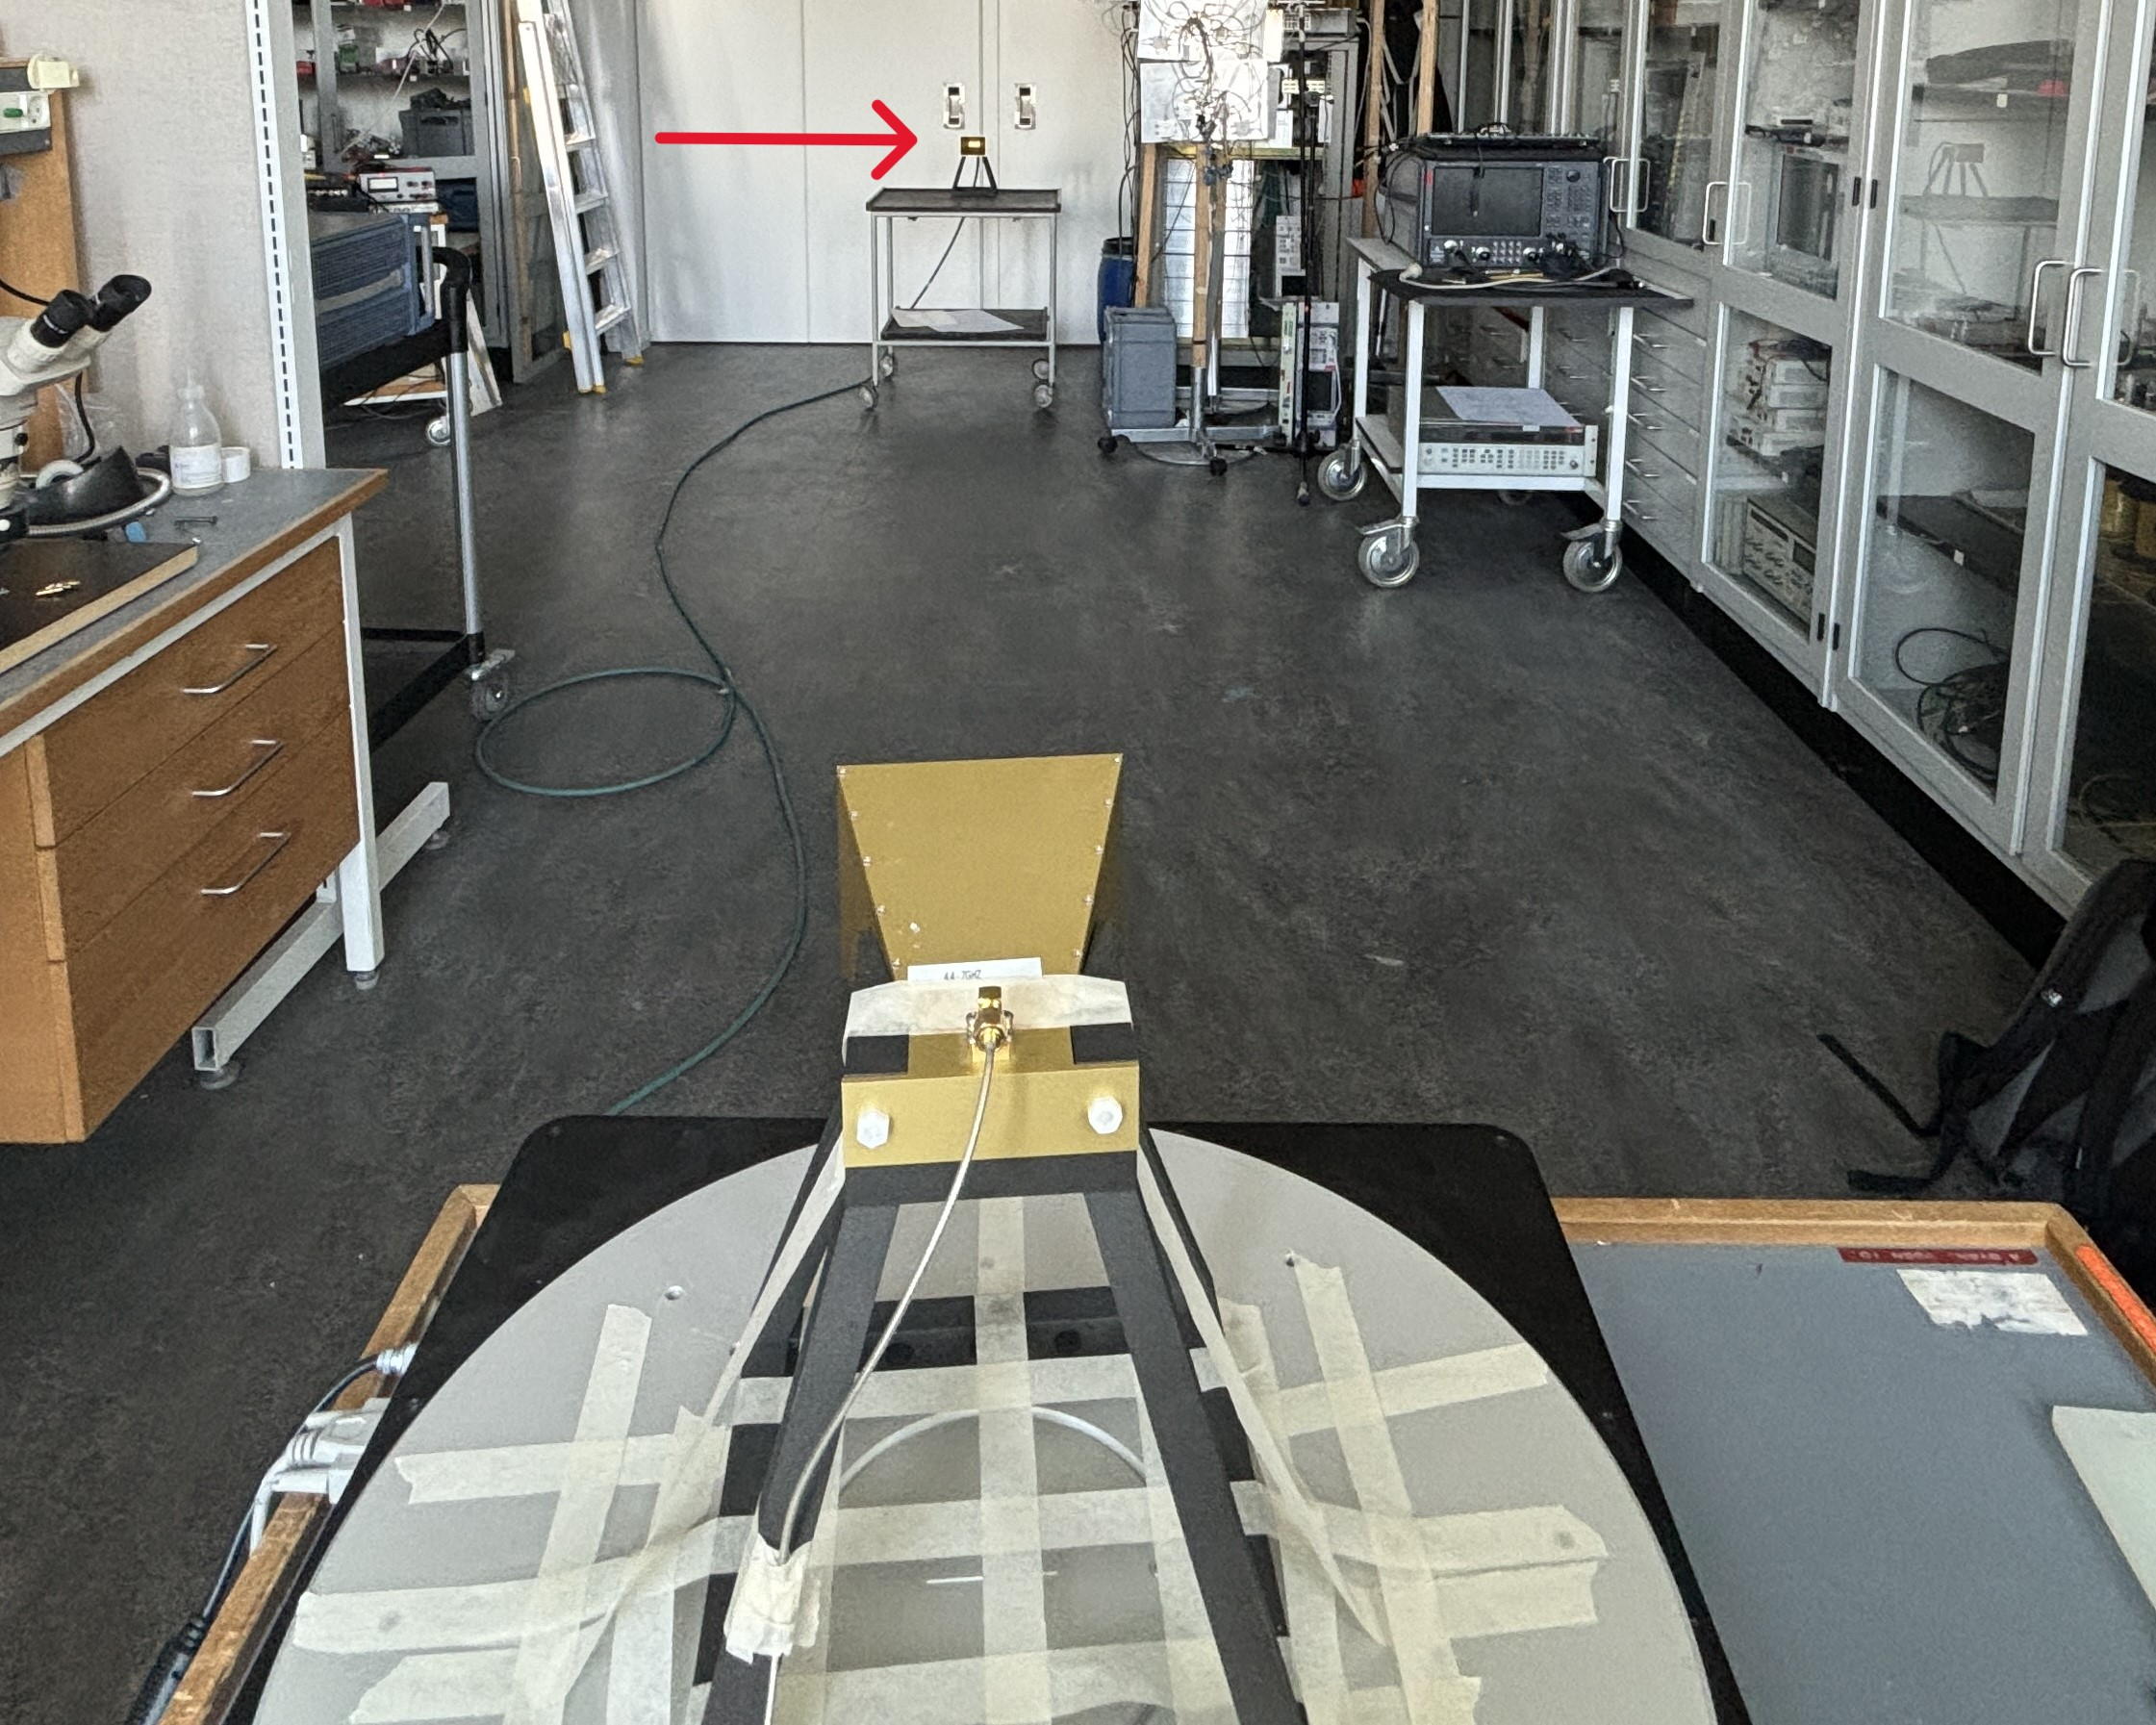
\includegraphics[width=0.7\textwidth]{figures/test_los_straight.JPG}
    \caption{View from receiver antenna at position \SI{50}{\degree} towards transmitter antenna.} \label{fig:a2_1}
\end{figure}

The test results can be found in table \ref{tab:a2_1a} and \ref{tab:a2_1b}.
\begin{table}[H]
    \centering
    \begin{tabular}{l|l|l|l}
        \multicolumn{4}{l}{\textbf{Frequency = 4.75 GHz}}         \\
        \hline
        \textbf{Position} & \multicolumn{3}{l}{\textbf{Power Measurement (dB)}} \\
        \textbf{(degrees)}  & Test 1    & Test 2  & Test 3  \\
        \hline
        \hline
        10      & -51.33    & -51.15    & -51.01 \\
        30      & \textcolor{red}{-46.82}    & \textcolor{red}{-46.63}    & \textcolor{red}{-46.52} \\
        50      & -46.96    & -46.77    & -46.66 \\
        70      & -49.07    & -48.88    & -48.78 \\
        90      & -55.30    & -55.18    & -48.78 \\
        110     & -70.33    & -69.99    & -69.81 \\
        130     & -67.82    & -67.30    & -67.27 \\
        150     & -66.85    & -66.73    & -66.58
        \end{tabular}
    \caption{Table of power measurements at each position repeated three times at frequency $f=\SI{4.75}{\giga\hertz}$. The maximum gain of each test is highlighted in red.}
    \label{tab:a2_1a}
\end{table}

\begin{table}[H]
    \centering
    \begin{tabular}{l|l|l|l}
        \multicolumn{4}{l}{\textbf{Frequency = 5.65 GHz}}         \\
        \hline
        \textbf{Position} & \multicolumn{3}{l}{\textbf{Power Measurement (dB)}} \\
        \textbf{(degrees)}  & Test 1    & Test 2  & Test 3  \\
        \hline
        \hline
        10      & -45.96    & -46.04    & -45.99 \\
        30      & -34.88    & -34.81    & -34.76 \\
        50      & \textcolor{red}{-31.05}    & \textcolor{red}{-30.99}    & \textcolor{red}{-30.93} \\
        70      & -34.61    & -34.56    & -34.51 \\
        90      & -49.59    & -49.54    & -49.47 \\
        110     & -64.89    & -64.79    & -64.67 \\
        130     & -50.16    & -50.15    & -50.15 \\
        150     & -58.68    & -58.68    & -58.79
        \end{tabular}
    \caption{Table of power measurements at each position repeated three times at frequency $f=\SI{5.65}{\giga\hertz}$. The maximum gain of each test is highlighted in red.}
    \label{tab:a2_1b}
\end{table}

\section{Corner-to-Corner Line-of-Sight}
The test is made with the antennas pointing directly towards each other from a skew angle in each their own corner of the room. The distance between the antennas is not measured. The start position is \SI{10}{\degree}, the end position is \SI{150}{\degree} and the increase is \SI{20}{\degree}. The following figure \ref{fig:a2_2} shows the setup:
\begin{figure}[H]
    \centering
    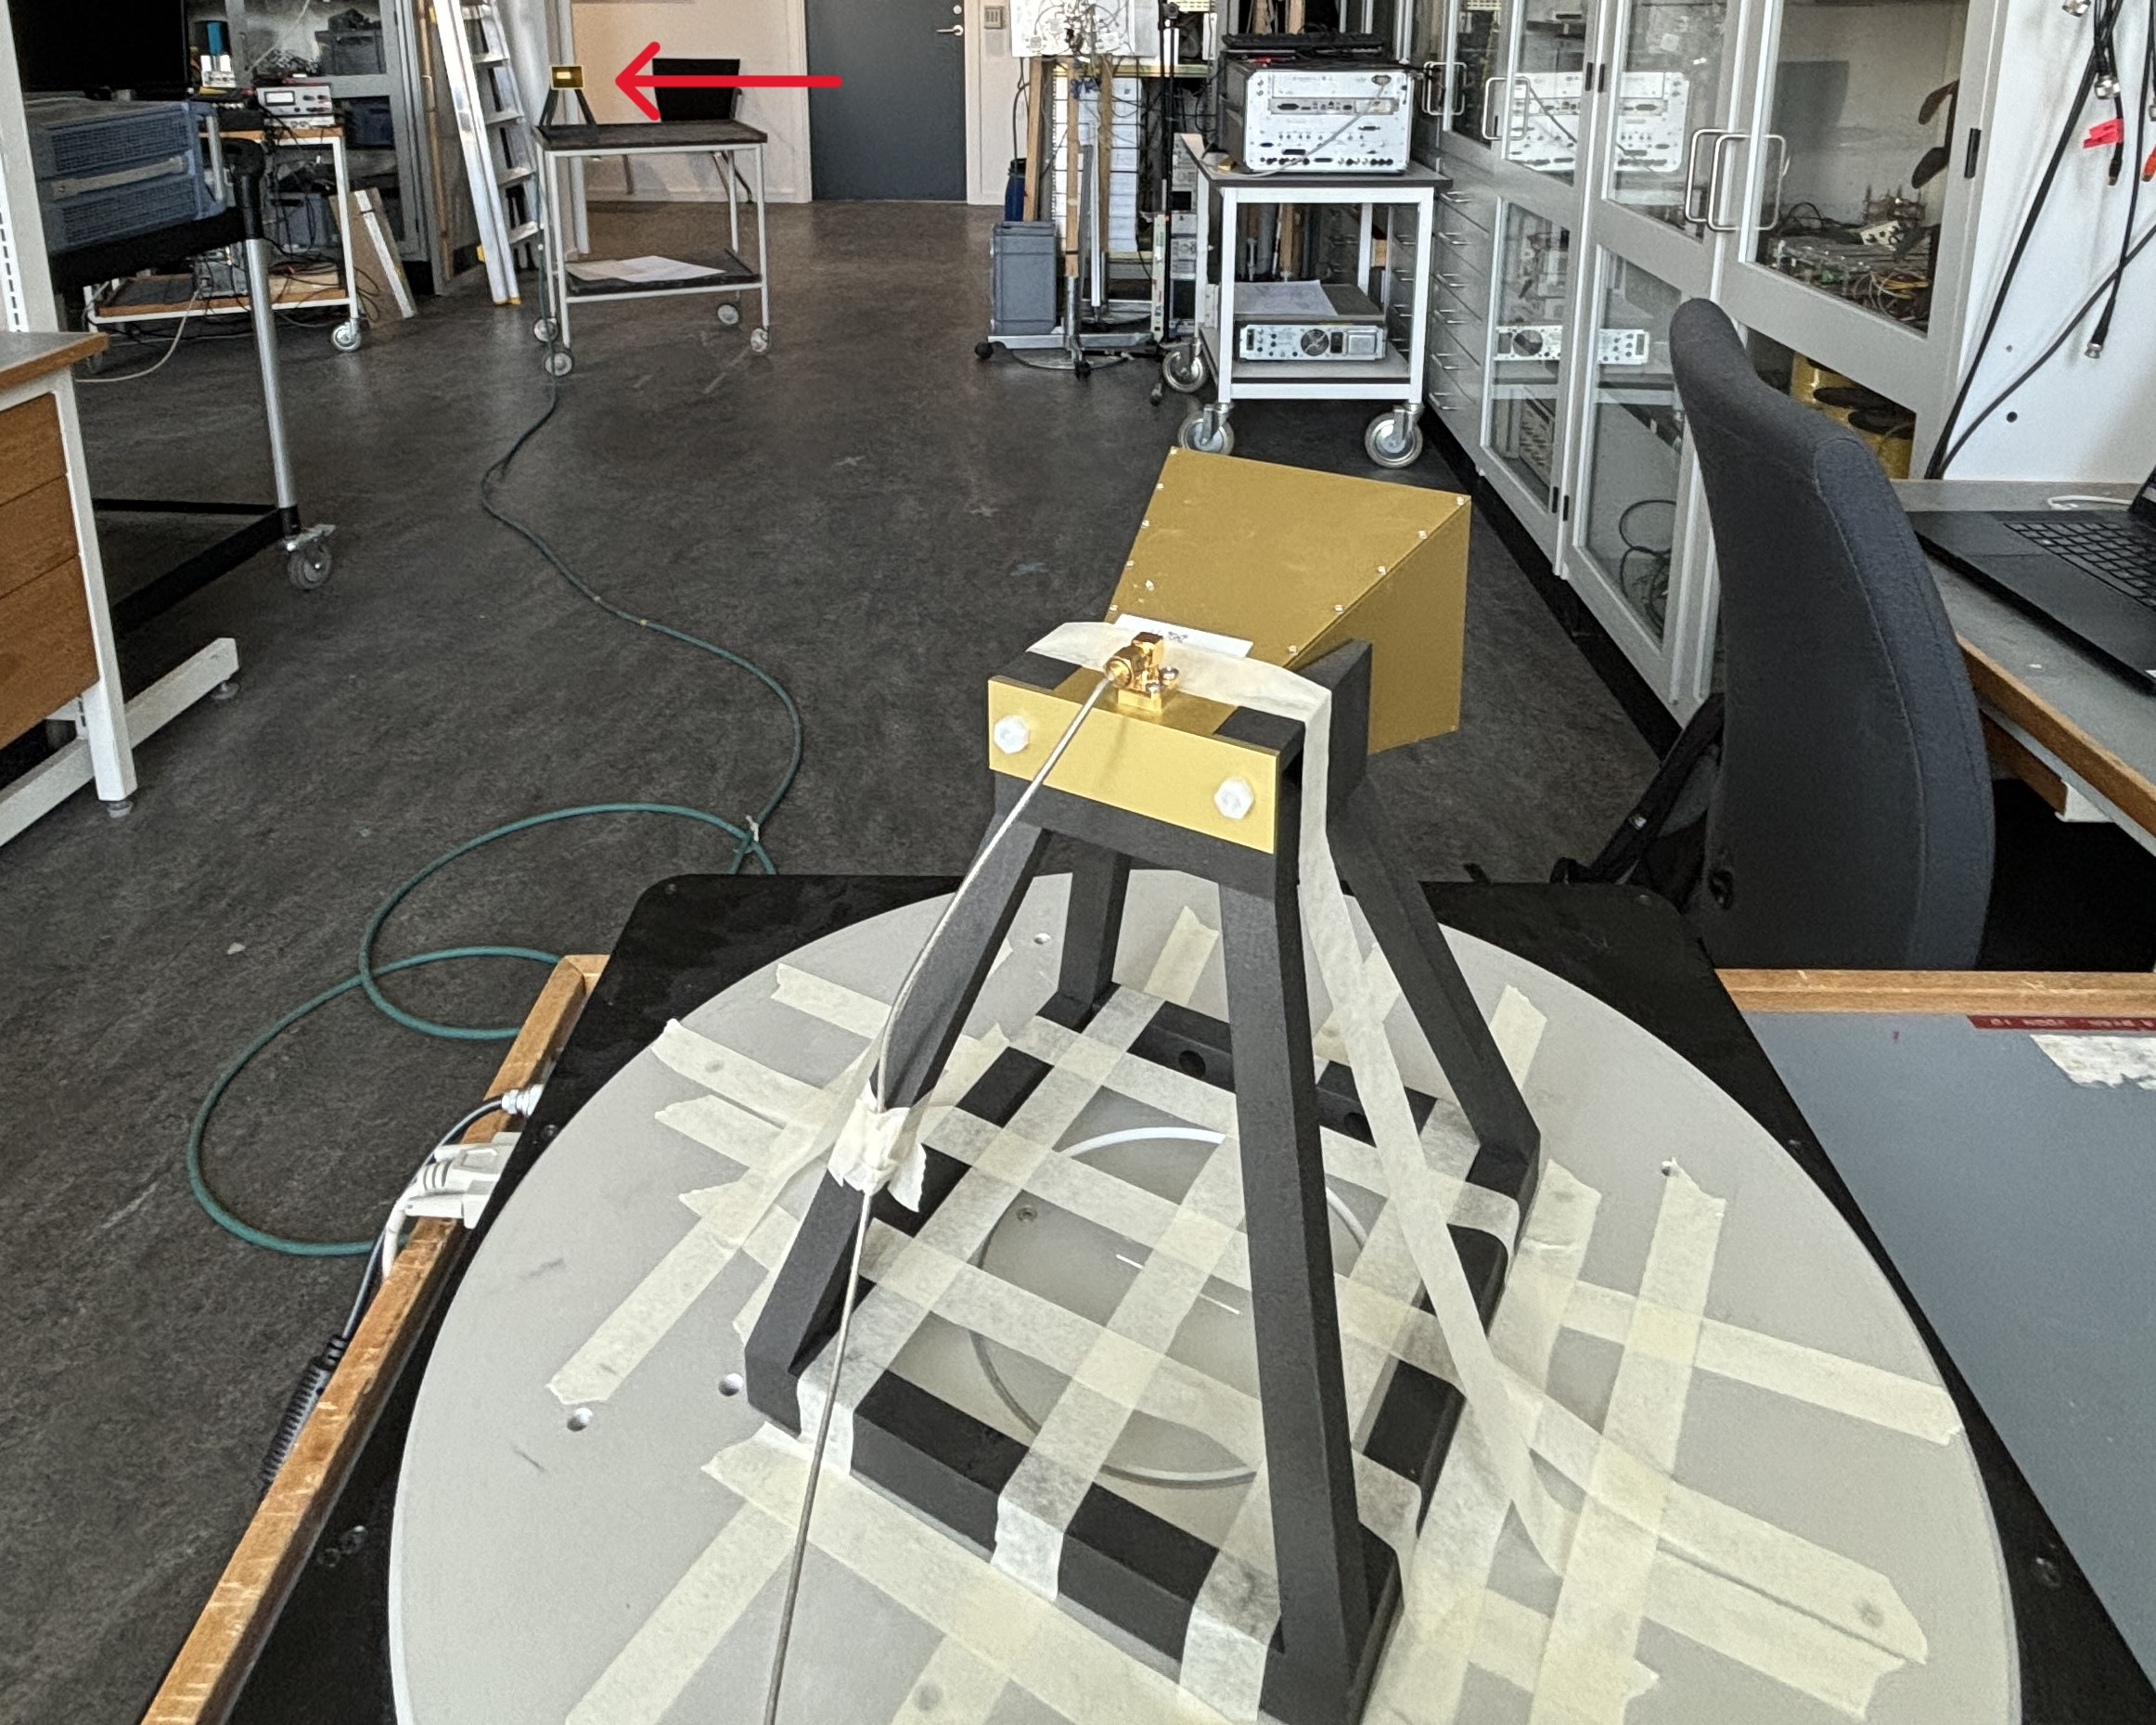
\includegraphics[width=0.7\textwidth]{figures/test_los_corner.JPG}
    \caption{View from receiver antenna at position \SI{10}{\degree} towards transmitter antenna.} \label{fig:a2_2}
\end{figure}

The test results can be found in table \ref{tab:a2_2a} and \ref{tab:a2_2b}.
\begin{table}[H]
    \centering
    \begin{tabular}{l|l|l|l}
        \multicolumn{4}{l}{\textbf{Frequency = 4.75 GHz}}         \\
        \hline
        \textbf{Position} & \multicolumn{3}{l}{\textbf{Power Measurement (dB)}} \\
        \textbf{(degrees)}  & Test 1    & Test 2  & Test 3  \\
        \hline
        \hline
        10      & -59.79    & -59.20    & -59.13 \\
        30      & -52.45    & -52.08    & -52.00 \\
        50      & -53.22    & -52.94    & -52.86 \\
        70      & \textcolor{red}{-48.34}    & \textcolor{red}{-48.11}    & \textcolor{red}{-48.06} \\
        90      & -51.32    & -51.09    & -51.04 \\
        110     & -70.33    & -58.41    & -58.33 \\
        130     & -75.39    & -75.27    & -75.29 \\
        150     & -62.40    & -62.15    & -62.07
        \end{tabular}
    \caption{Table of power measurements at each position repeated three times at frequency $f=\SI{4.75}{\giga\hertz}$. The maximum gain of each test is highlighted in red.}
    \label{tab:a2_2a}
\end{table}

\begin{table}[H]
    \centering
    \begin{tabular}{l|l|l|l}
        \multicolumn{4}{l}{\textbf{Frequency = 5.65 GHz}}         \\
        \hline
        \textbf{Position} & \multicolumn{3}{l}{\textbf{Power Measurement (dB)}} \\
        \textbf{(degrees)}  & Test 1    & Test 2  & Test 3  \\
        \hline
        \hline
        10      & -45.73    & -45.41    & -45.37 \\
        30      & -43.94    & -43.82    & -43.79 \\
        50      & -34.21    & -34.01    & -33.96 \\
        70      & \textcolor{red}{-32.29}    & \textcolor{red}{-32.15}    & \textcolor{red}{-32.10} \\
        90      & -37.35    & -37.27    & -37.23 \\
        110     & -51.65    & -51.62    & -51.63 \\
        130     & -68.07    & -68.20    & -68.02 \\
        150     & -56.72    & -56.73    & -56.66
        \end{tabular}
    \caption{Table of power measurements at each position repeated three times at frequency $f=\SI{5.65}{\giga\hertz}$. The maximum gain of each test is highlighted in red.}
    \label{tab:a2_2b}
\end{table}


\section{Antennas Perpendicular to Each Other}
The test is made with the transmitting antenna pointing Perpendicular to the receiver antenna. The distance between the antennas is $d=\SI{5.4}{\meter}$. The start position is \SI{10}{\degree}, the end position is \SI{150}{\degree} and the increase is \SI{20}{\degree}. The following figure \ref{fig:a2_3} shows the setup:
\begin{figure}[H]
    \centering
    \includegraphics[width=0.7\textwidth]{figures/test.JPG}
    \caption{View from receiver antenna at position \SI{50}{\degree} towards transmitter antenna.} \label{fig:a2_3}
\end{figure}

The test results can be found in table \ref{tab:a2_3a} and \ref{tab:a2_3b}.
\begin{table}[H]
    \centering
    \begin{tabular}{l|l|l|l}
        \multicolumn{4}{l}{\textbf{Frequency = 4.75 GHz}}         \\
        \hline
        \textbf{Position} & \multicolumn{3}{l}{\textbf{Power Measurement (dB)}} \\
        \textbf{(degrees)}  & Test 1    & Test 2  & Test 3  \\
        \hline
        \hline
        10      & -74.27    & -74.29    & -74.33 \\
        30      & -72.12    & -72.13    & -72.21 \\
        50      & -77.03    & -76.04    & -75.61 \\
        70      & -71.35    & -71.17    & -70.58 \\
        90      & -69.45    & -69.47    & -69.71 \\
        110     & \textcolor{red}{-68.42}    & \textcolor{red}{-68.28}    & \textcolor{red}{-68.15} \\
        130     & -79.83    & -80.25    & -79.30 \\
        150     & -75.04    & -75.25    & -75.23
        \end{tabular}
    \caption{Table of power measurements at each position repeated three times at frequency $f=\SI{4.75}{\giga\hertz}$. The maximum gain of each test is highlighted in red.}
    \label{tab:a2_3a}
\end{table}

\begin{table}[H]
    \centering
    \begin{tabular}{l|l|l|l}
        \multicolumn{4}{l}{\textbf{Frequency = 5.65 GHz}}         \\
        \hline
        \textbf{Position} & \multicolumn{3}{l}{\textbf{Power Measurement (dB)}} \\
        \textbf{(degrees)}  & Test 1    & Test 2  & Test 3  \\
        \hline
        \hline
        10      & -58.25    & -58.25    & -58.34 \\
        30      & -55.13    & -55.12    & -54.97 \\
        50      & \textcolor{red}{-49.13}    & \textcolor{red}{-49.11}    & \textcolor{red}{-49.08} \\
        70      & -52.44    & -52.40    & -52.43 \\
        90      & -50.17    & -50.10    & -50.10 \\
        110     & -49.77    & -49.73    & -49.81 \\
        130     & -52.26    & -52.20    & -52.26 \\
        150     & -58.72    & -59.04    & -58.64
        \end{tabular}
    \caption{Table of power measurements at each position repeated three times at frequency $f=\SI{5.65}{\giga\hertz}$. The maximum gain of each test is highlighted in red.}
    \label{tab:a2_3b}
\end{table}


\section{Straight Line-of-Sight with Table Intruder}




\section{Straight Line-of-Sight with Person Intruder}
